% !TEX root = main.tex
\appendix

\chapter{Λεπτομέρειες Υλοποίησης και Συμπληρωματικό Υλικό}
\label{chap:appendix}

\section{Κώδικας Πειραμάτων}
\label{sec:app-reproducibility}

Ο πηγαίος κώδικας της εργασίας βρίσκεται σε αύτο το  \href{https://github.com/AlkisPlas/langevin-sampling}{αποθετήριο}. Τα κεντρικά πειραματικά scripts είναι:

\begin{itemize}
  \item \texttt{experiments/run\_experiments.py}: εκτελεί τις $288 \times 20 = 5{,}760$
        αλυσίδες της μελέτης πλέγματος, παράγοντας το
        \texttt{results\_default\_<timestamp>.xlsx}.
  \item \texttt{experiments/run\_convergence.py}: εκτελεί τις $9 \times 10 = 90$
        αλυσίδες των $10^6$ επαναλήψεων στις βέλτιστες διαμορφώσεις, παράγοντας το
        \texttt{convergence\_<timestamp>.xlsx}.
  \item \texttt{experiments/aggregate\_seeds.py}: διαβάζει ένα xlsx ανά εκτέλεση
        και προσθέτει ένα φύλλο \texttt{aggregated} με διάμεσο, IQR, μέση τιμή
        και τυπικό σφάλμα ανά διαμόρφωση.
  \item \texttt{experiments/make\_thesis\_figures.py}: αναδημιουργεί
        όλα τα συγκεντρωτικά σχήματα του Κεφαλαίου~\ref{chap:experiments} από τα
        συγκεντρωτικά αρχεία xlsx.
  \item \texttt{experiments/make\_case\_study\_figures.py}: αναδημιουργεί
        τα trace plots, τα ACF και τα διαγράμματα καλής προσαρμογής της
        Ενότητας~\ref{sec:case-studies} επανεκτελώντας τις τέσσερις επιλεγμένες
        διαμορφώσεις.
\end{itemize}

Όλα τα scripts εξαρτώνται από τις βιβλιοθήκες \texttt{numpy}, \texttt{scipy},
\texttt{pandas}, \texttt{openpyxl} και \texttt{matplotlib}. Οι εκδόσεις πακέτων που
χρησιμοποιήθηκαν αναφέρονται στην Ενότητα~\ref{sec:exp-design} (υποενότητα Υλοποίηση).

\section{Ψευδοκώδικας Αλγορίθμων}
\label{sec:app-pseudo}

Οι τρεις δειγματολήπτες Langevin συνοψίζονται παρακάτω σε μορφή ψευδοκώδικα.
Η πλήρης Python υλοποίηση βρίσκεται στους φακέλους
\texttt{samplers/overdamped/ula/}, \texttt{samplers/overdamped/mala/} και
\texttt{samplers/underdamped/kinetic/splitting/baoab/} αντίστοιχα. Το σύνολο διαγνωστικών
είναι υλοποιημένο στο \texttt{metrics/comprehensive\_diagnostics.py}.

\subsection*{ULA --- Unadjusted Langevin Algorithm}

\begin{algorithmic}[1]
\Require βήμα $\eta > 0$, αριθμός βημάτων $N$, κλίση $\nabla U$, αρχικό $x_0$
\State $x \gets x_0$
\For{$k = 1, \ldots, N$}
  \State $\xi \sim \mathcal{N}(0, I_d)$
  \State $x \gets x - \eta\, \nabla U(x) + \sqrt{2\eta}\,\xi$
  \State Καταγραφή $X_k \gets x$
\EndFor
\end{algorithmic}

\subsection*{MALA --- Metropolis-Adjusted Langevin Algorithm}

\begin{algorithmic}[1]
\Require βήμα $\eta > 0$, $N$, $U$ και $\nabla U$, αρχικό $x_0$
\State $x \gets x_0$; $a \gets 0$
\For{$k = 1, \ldots, N$}
  \State $\xi \sim \mathcal{N}(0, I_d)$
  \State $x' \gets x - \eta\, \nabla U(x) + \sqrt{2\eta}\,\xi$
  \State $\log r \gets U(x) - U(x') + \frac{1}{4\eta}\bigl(\|x' - x + \eta\nabla U(x)\|^2 - \|x - x' + \eta\nabla U(x')\|^2\bigr)$
  \State $u \sim \mathrm{Uniform}(0,1)$
  \If{$\log u < \log r$}
    \State $x \gets x'$; $a \gets a + 1$
  \EndIf
  \State Καταγραφή $X_k \gets x$
\EndFor
\State Ποσοστό αποδοχής $\gets a / N$
\end{algorithmic}

\subsection*{BAOAB --- Underdamped Langevin (Splitting Ολοκληρωτής)}

\begin{algorithmic}[1]
\Require βήμα $\eta$, τριβή $\gamma$, $N$, $\nabla U$, αρχικό $(x_0, v_0)$
\State $x, v \gets x_0, v_0$
\State $a \gets \exp(-\gamma\eta)$, $s \gets \sqrt{1 - a^2}$
\For{$k = 1, \ldots, N$}
  \State $v \gets v - \tfrac{\eta}{2}\,\nabla U(x)$ \Comment{B}
  \State $x \gets x + \tfrac{\eta}{2}\, v$ \Comment{A}
  \State $\xi \sim \mathcal{N}(0, I_d)$; $v \gets a\, v + s\, \xi$ \Comment{O}
  \State $x \gets x + \tfrac{\eta}{2}\, v$ \Comment{A}
  \State $v \gets v - \tfrac{\eta}{2}\,\nabla U(x)$ \Comment{B}
  \State Καταγραφή $X_k \gets x$
\EndFor
\end{algorithmic}

\section{Σύνολο Διαγνωστικών}
\label{sec:app-metrics}

Παραθέτουμε τους υπολογισμούς διαγνωστικών του
Κεφαλαίου~\ref{chap:experiments}, όπως υλοποιούνται στο
\texttt{metrics/comprehensive\_diagnostics.py}.

\paragraph{Αποτελεσματικό μέγεθος δείγματος (ESS).}
Για κάθε συντεταγμένη $k$, υπολογίζεται η αμερόληπτη αυτοσυσχέτιση μέσω FFT
$\hat\rho(\ell)$ έως lag $L = \min(N/2, 500)$. Χρησιμοποιείται ο εκτιμητής
αρχικής θετικής ακολουθίας του \citet{geyer1992practical}: ξεκινώντας με
$\hat\tau = 1$, συσσωρεύεται $\hat\tau \gets \hat\tau + 2\hat\rho(\ell)$
όσο $\hat\rho(\ell) > 0.05$. Το ESS ανά συντεταγμένη είναι
$\hat n_\mathrm{eff} = N / \hat\tau$. Το αναφερόμενο \texttt{ess\_mean}
είναι ο μέσος όρος ανά συντεταγμένη. \texttt{ess\_min} και
\texttt{ess\_max} είναι τα ακραία ανά συντεταγμένη.

\paragraph{Quantile MAE.}
Για κάθε συντεταγμένη $k$ και κάθε επίπεδο $q \in \{0.025, 0.5, 0.975\}$,
υπολογίζεται το εμπειρικό $q$-ποσοστημόριο $\hat F_k^{-1}(q)$ μέσω
\texttt{numpy.percentile} και το θεωρητικό $q$-ποσοστημόριο
$F_k^{-1}(q)$ μέσω της αναλυτικής αντίστροφης CDF της περιθώριας κατανομής.
Αναφέρεται ο μέσος όρος ανά συντεταγμένη του μέσου ανά $q$ του
$|\hat F_k^{-1}(q) - F_k^{-1}(q)|$.

\paragraph{Λόγος κάλυψης ουράς.}
Για κάθε συντεταγμένη $k$ και κάθε επίπεδο $q \in \{0.01, 0.05, 0.95,
0.99\}$, έστω $\theta = F_k^{-1}(q)$. Για $q < 0.5$, υπολογίζεται
$c = \frac{1}{N}\sum_{t=1}^N \mathbf{1}\{X_t^{(k)} \leq \theta\}$.
Για $q > 0.5$, $c = \frac{1}{N}\sum_{t=1}^N \mathbf{1}\{X_t^{(k)} \geq
\theta\}$. Η αναμενόμενη τιμή του $c$ υπό ακριβή δειγματοληψία είναι
$\min(q, 1-q)$. Αναφέρεται ο λόγος $c / \min(q, 1-q)$.

\paragraph{Στατιστική Kolmogorov--Smirnov.}
Για κάθε συντεταγμένη $k$, υπολογίζεται
$D_n^{(k)} = \sup_x |\hat F_k(x) - F_k(x)|$ χρησιμοποιώντας
\texttt{scipy.stats.kstest} έναντι της αναλυτικής CDF περιθώριας κατανομής.
Αναφέρεται ο μέσος όρος ανά συντεταγμένη ως \texttt{ks\_stat\_mean}.
Διατηρείται μόνο η στατιστική του ελέγχου. Η αντίστοιχη $p$-τιμή δεν ερμηνεύεται
ορθά παρουσία αυτοσυσχέτισης και δεν αναφέρεται.

\paragraph{Ποσοστό απόκλισης.}
Κλάσμα δειγμάτων (μετά το burn-in) για τα οποία οποιαδήποτε συντεταγμένη
υπερβαίνει το $10^6$ σε απόλυτη τιμή. Χρησιμοποιείται ως έλεγχος αριθμητικής
σταθερότητας.

\paragraph{Μεροληψίες ροπών.}
$\left|\hat\mu_k - \mu_k\right|$ και $\left|\hat\sigma_k^2 -
\sigma_k^2\right|$ κατά μέσο όρο ανά συντεταγμένη, όπου $\mu_k$ και
$\sigma_k^2$ είναι η αναλυτική μέση τιμή και διακύμανση της περιθώριας
κατανομής. Για την κατανομή Cauchy αυτές είναι αόριστες και αναφέρονται ως
\texttt{NaN}.

\section{Πλήρη Αποτελέσματα Μελέτης Πλέγματος}
\label{sec:app-results-table}

Το πλήρες βιβλίο εργασίας της μελέτης πλέγματος
\texttt{experiments/results/original\_thesis/results\_default\_20260525\_104845\_agg.xlsx}
έχει τρία κύρια φύλλα. Το φύλλο \texttt{summary} περιέχει μία γραμμή ανά
(διαμόρφωση, εκτέλεση), δίνοντας $5{,}760$ γραμμές με $43$ στήλες. Το φύλλο
\texttt{aggregated} περιέχει μία γραμμή ανά διαμόρφωση ($288$ γραμμές),
με τέσσερις στήλες ανά μετρική: \texttt{<metric>\_central},
\texttt{<metric>\_low}, \texttt{<metric>\_high},
\texttt{<metric>\_n\_valid}. Η κεντρική στήλη δίνει είτε τη διάμεσο
(για μετρικές ανθεκτικές στη λοξότητα: KS, quantile-MAE και
κάλυψη ουράς) είτε τον μέσο όρο (για ESS, ποσοστό αποδοχής και μεροληψία ροπών).
Οι χαμηλές και υψηλές στήλες δίνουν το IQR (για διάμεσο) ή τη ζώνη τυπικού
σφάλματος (για μέσο όρο). Το φύλλο \texttt{per\_dim} παρέχει ανάλυση ανά συντεταγμένη.

Το πλήρες σύνολο στηλών μετρικών στο φύλλο ανά εκτέλεση είναι:

\begin{itemize}
\item \textbf{Διαμόρφωση}: \texttt{algorithm}, \texttt{distribution},
      \texttt{d}, \texttt{eta}, \texttt{gamma}, \texttt{nu},
      \texttt{n\_steps}, \texttt{burn\_in}, \texttt{seed}.
\item \textbf{Κόστος}: \texttt{runtime\_seconds}, \texttt{ess\_per\_sec},
      \texttt{n\_samples\_post}.
\item \textbf{Ειδικά δειγματολήπτη}: \texttt{acceptance\_rate} (MALA),
      \texttt{divergence\_rate}.
\item \textbf{Ανάμειξη}: \texttt{ess\_mean}, \texttt{ess\_min},
      \texttt{ess\_max}, \texttt{ess\_ratio\_mean}, \texttt{iat\_mean},
      \texttt{acf\_lag\_1}, \texttt{acf\_lag\_10}, \texttt{acf\_lag\_50},
      \texttt{acf\_lag\_100}.
\item \textbf{Ροπές}: \texttt{empirical\_mean\_avg},
      \texttt{theoretical\_mean\_avg}, \texttt{mean\_abs\_bias},
      \texttt{empirical\_var\_avg}, \texttt{theoretical\_var\_avg},
      \texttt{var\_abs\_bias}, \texttt{empirical\_std\_avg},
      \texttt{empirical\_median\_avg},
      \texttt{theoretical\_median\_avg},
      \texttt{median\_abs\_bias}.
\item \textbf{Προσαρμογή κατανομής}: \texttt{quantile\_mae\_avg},
      \texttt{quantile\_mae\_q0.025}, \texttt{quantile\_mae\_q0.5},
      \texttt{quantile\_mae\_q0.975}, \texttt{tail\_cov\_ratio\_q0.01},
      \texttt{tail\_cov\_ratio\_q0.05}, \texttt{tail\_cov\_ratio\_q0.95},
      \texttt{tail\_cov\_ratio\_q0.99}, \texttt{ks\_stat\_mean}.
\end{itemize}

Το φύλλο $\texttt{per\_dim}$ παρέχει ανάλυση ανά συντεταγμένη για κάθε
μετρική για την οποία ο υπολογισμός ανά συντεταγμένη έχει νόημα.

\section{Αποτελέσματα Μελέτης Σύγκλισης}
\label{sec:app-convergence-table}

Ο πλήρης πίνακας της μελέτης σύγκλισης βρίσκεται στο
\texttt{experiments/results/original\_thesis/convergence\_20260525\_122341.xlsx} στο
φύλλο \texttt{convergence\_summary} (γραμμές ανά εκτέλεση) και στο φύλλο
\texttt{aggregated} (διάμεσοι και IQR ανά σημείο ελέγχου). Κάθε μία από
τις $9$ αλυσίδες (αλγόριθμος, κατανομή) επαναλαμβάνεται $10$ φορές ανεξάρτητα
και αξιολογείται στα τέσσερα σημεία ελέγχου
$N \in \{5\!\cdot\!10^4, 10^5, 5\!\cdot\!10^5, 10^6\}$.
Ο Πίνακας~\ref{tab:app-ks-conv} δίνει τη διάμεσο KS σε κάθε σημείο ελέγχου.

\begin{table}[ht]
\centering
\small
\begin{tabular}{lccccc}
\toprule
Αλγόριθμος \& Κατανομή-Στόχος & $N = 5\!\cdot\!10^4$ & $N = 10^5$ & $N = 5\!\cdot\!10^5$ & $N = 10^6$ & Λόγος \\
\midrule
ULA Gaussian                  & $0.0093$ & $0.0124$ & $0.0063$ & $0.0055$ & $0.58$ \\
ULA Student-$t$               & $0.0128$ & $0.0135$ & $0.0077$ & $0.0067$ & $0.52$ \\
ULA Cauchy                    & $0.0330$ & $0.0301$ & $0.0270$ & $0.0246$ & $0.75$ \\
MALA Gaussian                 & $0.0057$ & $0.0038$ & $0.0015$ & $0.0010$ & $0.18$ \\
MALA Student-$t$              & $0.0053$ & $0.0039$ & $0.0019$ & $0.0010$ & $0.19$ \\
MALA Cauchy                   & $0.0170$ & $0.0124$ & $0.0071$ & $0.0046$ & $0.27$ \\
BAOAB Gaussian                & $0.0043$ & $0.0035$ & $0.0012$ & $0.0008$ & $0.18$ \\
BAOAB Student-$t$             & $0.0057$ & $0.0046$ & $0.0022$ & $0.0018$ & $0.31$ \\
BAOAB Cauchy                  & $0.0202$ & $0.0179$ & $0.0142$ & $0.0108$ & $0.53$ \\
\bottomrule
\end{tabular}
\caption{Διάμεσος της στατιστικής Kolmogorov--Smirnov σε κάθε σημείο ελέγχου
της μελέτης σύγκλισης, μαζί με τον λόγο μεταξύ της τιμής στο $N = 10^6$
και της τιμής στο $N = 5\!\cdot\!10^4$. Ο κλασικός ρυθμός $1/\sqrt n$ για
μια αλυσίδα που στοχεύει σωστά στην $\pi$ είναι $0.224$. Οι διάμεσοι
υπολογίζονται επί $10$ ανεξάρτητων εκτελέσεων.}
\label{tab:app-ks-conv}
\end{table}

\section{Συμπληρωματικά Σχήματα}
\label{sec:app-figures}

\subsection{Σύγκλιση Quantile-MAE}
\label{sec:app-fig-qmae}

Το Σχήμα~\ref{fig:app-qmae} αναπαράγει το Σχήμα~\ref{fig:qmae-conv}
για αναφορά. Παραλείπεται η εκτεταμένη συζήτηση (βλ.
Ενότητα~\ref{sec:convergence-study}).

\begin{figure}[ht]
\centering
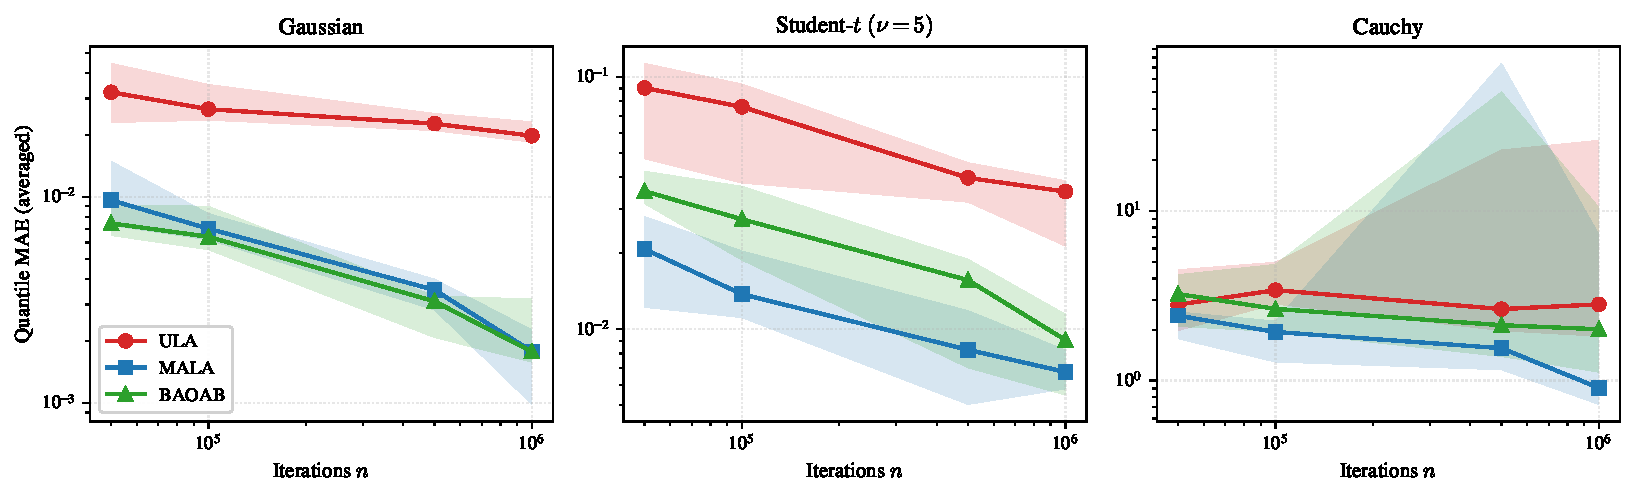
\includegraphics[width=\textwidth]{../../experiments/figures/original_thesis/quantile_mae_convergence}
\caption{Μέσο quantile MAE συναρτήσει $N$, αναπαραγόμενο από το
Σχήμα~\ref{fig:qmae-conv}.}
\label{fig:app-qmae}
\end{figure}

\subsection{Ιστόγραμμα Ποσοστών Αποδοχής Βέλτιστης Διαμόρφωσης}
\label{sec:app-fig-accept}

Το Σχήμα~\ref{fig:app-accept} (= Σχήμα~\ref{fig:mala-accept})
δείχνει πώς μεταβάλλεται το ποσοστό αποδοχής του MALA με το βήμα και τη
διάσταση. Από εδώ προκύπτει η σύσταση για ζώνη $0.5$--$0.85$ για $d \leq 10$.

\begin{figure}[ht]
\centering
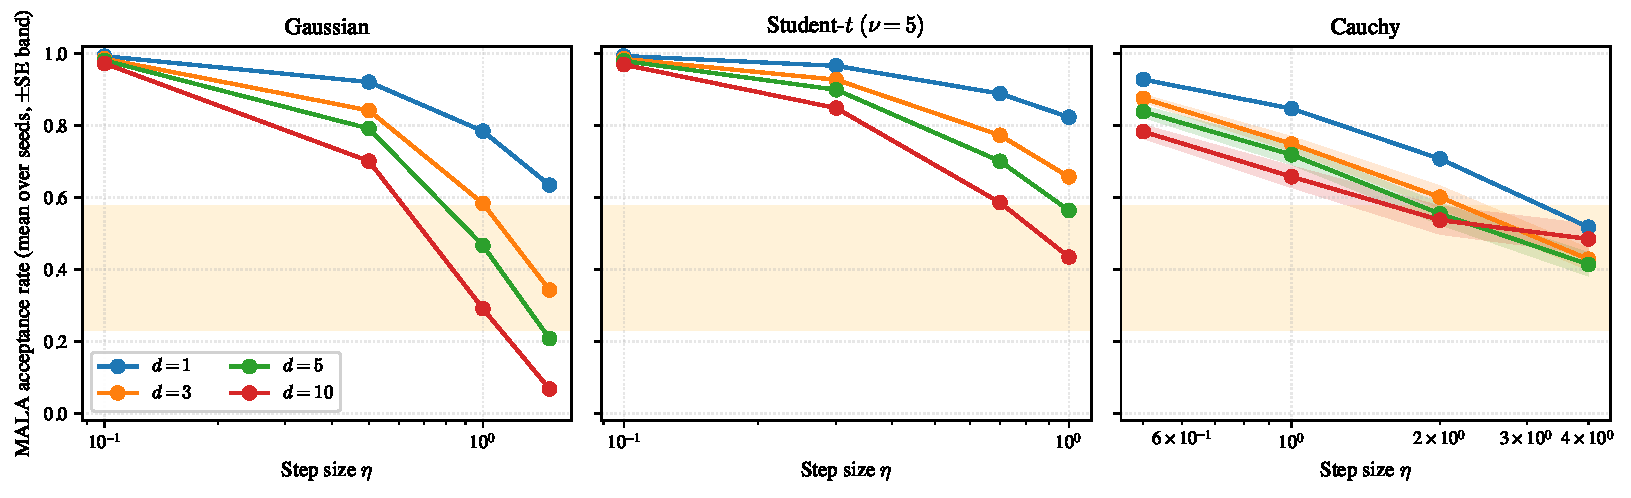
\includegraphics[width=\textwidth]{../../experiments/figures/original_thesis/mala_acceptance}
\caption{Ποσοστό αποδοχής MALA ως συνάρτηση του βήματος και της διάστασης
(επαναλαμβάνεται από την Ενότητα~\ref{sec:grid-study} για τη συζήτηση των
συμπερασμάτων).}
\label{fig:app-accept}
\end{figure}
